%Folgende Zeile aktivieren und als SVN property "svn:keywords" auf "Id" setzen, um SVN Versionsinformationen im Dokument zu erhalten
%\svnInfo $Id: einleitung.tex 60 2012-01-26 15:56:06Z koppor $ 

\chapter{2D - Verfahren}
\label{chap:2d}
	\section{SIFT/SURF}
		SIFT (Scale-invariant feature transform) ist ein von David Lowe 1999 vorgestelltes Verfahren zur Extraktion von lokalen Merkmalen aus Bildern. Die mit diesem Verfahren gefundene Merkmale haben die Eingeschaft, dass sie robust gegenüber Rotation, Translation und Skalierung sind, und damit zuverlässig in anderen Bilder wiedererkannt werden können.
Um Objekte in Bildern mit SIFT erkennen und lokalisieren zu können, sind also zwei Schritte nötig:
\begin{enumerate}
	\item Extraktion und Beschreibung von Merkmalen (Features) des gesuchten Objekts
	\item Lokalisation der Merkmale im Suchbild
\end{enumerate}

\subsection{Extraktion und Beschreibung von Merkmalen (Features) des gesuchten Objekts}
Der Algorithmus zur Extraktion und Beschreibung der Merkmale besteht dabei aus vier Verarbeitungsstufen:
	\subsubsection{Ermittlung potentieller Merkmale in DoG-Pyramiden}
		Um Merkmale zu ermitteln, die robust gegenüber Skalierung sind, kommt das Verfahren der DoG (Difference of gaussians) Pyramiden zum Einsatz. Dabei werden aus dem Ausgangsbild zunächst n Gaußpyramiden berechnet. Eine Pyramide besteht dabei aus fortlaufen stärker geglätteten Bildern des Ausgangsbildes $g$. Zur Glättung kommt dabei ein Gaußfilter $G$ zum Einsatz:
\begin{equation*}
 g(x, y) * G_\vartheta (x, y) = g(x, y) * (\frac{1}{\sqrt{2\pi \vartheta ^2}}\cdot e^{-\frac{x^2 + y^2}{2\vartheta ^2}})
\end{equation*}

Im Anschluss wird das letzte Bild der Pyramide um 50\% verkleinert, und daraus durch erneute fortlaufende Glättung mit dem Gaußfilter eine neue Pyramide erzeugt.
Je zwei benachbarte Bilder einer Gaußpyramide werden nun voneinander Subtrahiert. Aus den Resultaten entstehen dabei die DoG Pyramiden:
\begin{figure}
  \begin{center}
    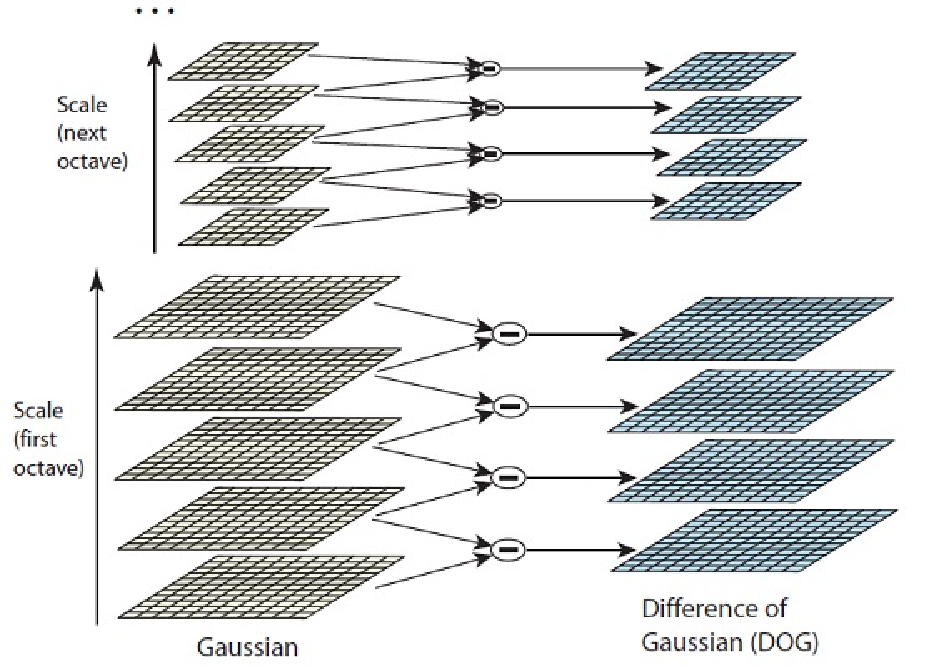
\includegraphics[width=\textwidth]{dog.pdf}
    \caption{DoG-Pyramiden}
    \label{fig:dog_pyr}
  \end{center}
\end{figure}

Die dadurch erzeugten DoG-Pyramiden werden nun auf minimale und maximale Pixelwerte untersucht.
Ein Maximum ist gefunden, wenn der Grauwert eines Pixels größer als der seiner 26 Nachbarn ist. Nachbarschaft eines Pixels ergibt sich dann aus seinen acht Nachbarn der selben Ebene, sowie aus den jeweils neun Nachbarn der benachbarten Ebenen in der DoG-Pyramide.
Die Suche nach Minima erfolg auf die selbe Art und Weise. Die Information, auf welcher Skalierung die potentiellen Merkmalspunkte liegen, wird dabei ebenfalls gespeichert.
\begin{figure}[H]
  \begin{center}
    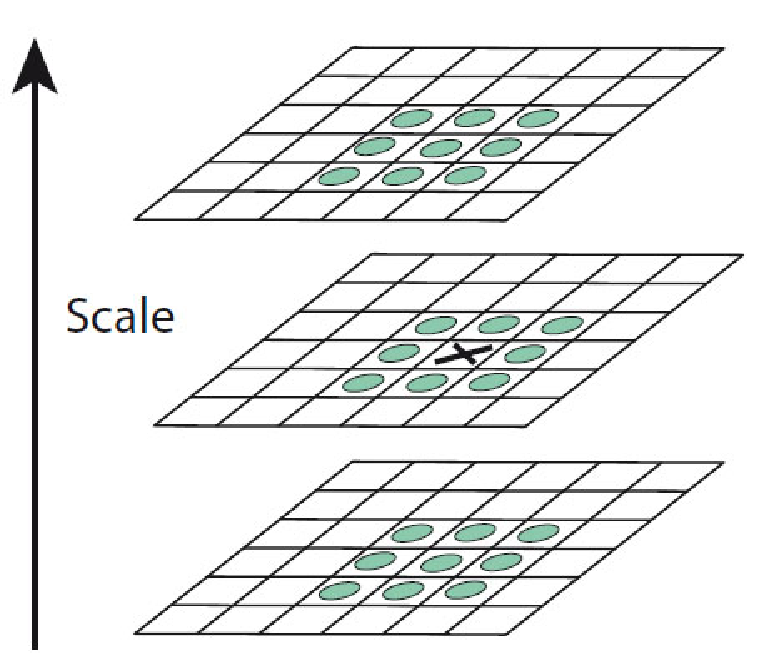
\includegraphics[width=0.5\textwidth]{scale.pdf}
    \caption{Nachbarschaft eines Pixels}
    \label{fig:neighbor}
  \end{center}
\end{figure}
	\subsubsection{Filterung und Lokalisation potentieller Merkmalspunkte}
		Das oben genannte Verfahren liefert neben den robusten Merkmalspunkten eine große Menge von instabilen, für die weitere Verarbeitung nicht zu gebrauchende Merkmale.
Daher werden die gefundenen Merkmalspunkte anhand von Stabilitätskriterien gefiltert.
Im ersten Schritt werden dabei alle Merkmalspunkte entfernt, die einen DoG-Wert von weniger als 0,03, und somit einen relativ niedrigen Kontrast besitzen.
Merkmalspunkte, die auf Ecken liegen sind “prägnanter” (und somit staibler) als solche, die auf einer Kante liegen, daher werden alle Merkmalspunkte entfernt, die auf einer Kante, aber nicht auf einer Ecke liegen.
Dies geschieht unter Anwendung der Hesse-Matrix (todo).
	\subsubsection{Bestimmung der Hauptorientierungen}
		Um Invarianz der verbleibenden Merkmalspunkte gegenüber Rotation zu erreichen, wird für jeden Merkmalspunkt dessen Hauptorientierung berechnet.
Dafür nutzt man das gaußgefilterte Bild, welches der Skalierung des zu untersuchenden Merkmalspunktes am nächsten kommt. In diesem Bild werden nun innerhalb einer festen Region um den Merkmalspunkt herum die Gradientenlängen $m(x, y)$ und die Gradientenorientierungen $\theta (x, y)$ bezüglich eines Punktes $g(x, y)$ berechnet, wobei
\begin{equation*}
m(x, y) = \sqrt{(g(x + 1, y) - g(x - 1, y))^2 +(g(x, y+1) - g(x, y-1))^2}
\end{equation*}

und

\begin{equation*}
\theta (x, y) = tan^{-1}\cdot \frac{g(x +1, y) - g(x-1, y)}{g(x, y +1) - g(x, y-1)}
\end{equation*}

Die so ermittelten Gradientenorientierungen werden nun anhand ihrer Gradientenlängen gewichtet. Dadurch haben Gradientenrichtungen mit großer Gradientenlänge einen größeren Einfluss auf die Hauptorientierung als Gradientenrichtungen mit niedriger Gradientenlänge.
Danach werden die Gradientenorientierungen zusätzlich anhand ihrer Entfernung zum Merkmalspunkt gewichtet, um Gradientenrichtungen, die sich näher am Merkmalspunkt befinden stärker zu gewichten.

Aus den gewichteten Gradientenorientierungen wird nun ein Orientierungshistogramm erstellt. Dieses Histogramm ist in 36 Winkelbereiche eingeteilt und hat somit eine Klassenbreite von $10\,^{\circ}$.
Jede Gradientenorientierung wird dabei anhand ihrer Gewichtung an der passenden Stelle im Histogramm aufaddiert. \\
Nach der Erstellung des Histogramms kann aus diesem die Gradientenlänge $m_{max}$ abgelesen werden (Winkelbereich mit der größten Summe). Die Hauptorientierung des Merkmalspunktes  setzt sich dabei aus $m_{max}$, sowie der zugehörigen Gradientenorientierung $\theta_{max}$ maxzusammen.
Für den Fall, dass eine weitere Orientierung mit der Gradientenlänge $m_i > 0,8 m_{max}$
existiert; wie es bei Eckpunkten häufig der Fall ist; wird an der Stelle $(x, y)$ ein weiterer Merkmalspunkt mit der Hauptorientierung $(m_i, \theta_i)$ erstellt.
\subsection{Lokalisation der Merkmale im Suchbild}
Wurden nun im ersten Schritt die robusten Merkmale des gesuchten Objekts extrahiert, können diese im Suchbild wiedererkannt werden.
Dies geschieht, in dem man die extrahierten Merkmale des Objekts mit denen im Suchbild auf Übereinstimmung hin untersucht.
Dafür existieren verschiedene Ansätze.
	\subsubsection{Merkmalsvergleich anhand des eukllidischen Abstands}
Der einfachste Ansatz zwei Deskriptoren miteinander zu Vergleichen, ist die Bestimmung des euklidischen Abstands der Merkmalsvektoren
\begin{equation*}
e = \sqrt{\sum_{i = 1}^{n}(V_{1i} - V_{2i})}
\end{equation*}


